	\textit{\small Note: full source code is at the end of this document.}
	\subsection{Python, Primary Programming Language}
	
	\par Python is an interpreted, interactive, object-oriented programming language. It incorporates modules, exceptions, dynamic typing, very high-level dynamic data types, and classes. Python combines remarkable power with very clear syntax. It has interfaces to many system calls and libraries, as well as to various window systems, and is extensible in C or C++. It is also usable as an extension language for applications that need a programmable interface. Finally, Python is portable: it runs on many Unix variants, on the Mac, and on Windows 2000 and later.
	\par We will use Python to control each module via the coordinator XBee module that will be attached to a PC. Its versatility provides the ability to interface lower level controls on the XBee with a high level graphical interface all in one language. 
	\par A readily available python package allows for easy interfacing with the camera unit. This package provides a pure Python interface to the Raspberry Pi camera module for Python 2.7 (or above) or Python 3.2 (or above). It can configure resolution and give different dimensions to the video or picture files. It can also take photos under varying conditions if given the right parameters for a camera to take a good picture in a variety of different conditions including poor lighting. 
	The code for the camera is as follows:
	\begin{lstlisting}
	# A test of the cameras functions
	from time import sleep
	from picamera import PiCamera
	
	camera = PiCamera()
	camera.capture('/home/pi/Desktop/test.jpg')  #saves camera picture to file location specified
	
	
	# Camera trigger implementations
	import RPi.GPIO as GPIO
	from picamera import PiCamera
	from time import sleep
	GPIO.setmode(GPIO.BOARD)
	GPIO.setup(16, GPIO.IN, pull_up_down=GPIO.PUD_DOWN) #Pull down to make pin read active high
	GPIO.input(16) #pin 16 being read
	if GPIO.input(16):
	camera = PiCamera()
	camera.capture('/home/pi/Desktop/test.jpg')
	print('input high/camera on')
	else:
	camera = PiCamera()
	camera.capture('/home/pi/Desktop/testfail.jpg')
	print('input low/camera off')
	GPIO.cleanup()
	\end{lstlisting}
	\subsubsection{Explanation of Raspberry Pi Code Functions}
		\noindent\textbf{The audiotest.py decsription: }
		\par This code establishes the audio streaming parameters to properly record and retain the data one has to set various parameters such as the resolution and sampling rate of the audio stream. This code records audio via a USB audio recording device and is set to record for 30 seconds. This then saves the file under the name test1.wav and will be placed in the main directory of the raspberry pi. \\
		
		\noindent\textbf{ The devicecheck.py description:}
		\par This code just checks to see what USB audio devices are connected and recognized by the python pyaudio module. It should return the device name and what channel it is occupying. This information is needed to help set up the rest of the parameters in the audiotest.py code.\\
		
		\noindent\textbf{ The cameratrigger.py description:}
		\par This code demonstrates how the general purpose input and output pins on the raspberry pi would have been implemented to read active high on pin 16 to be able to receive a signal from the Xbee device. When the pin receives 3.3V from the XBee device then the camera will trigger and take a picture and save it in the file directory specified. \\
		
		\noindent\textbf{ The cameratest.py description:}
		\par Simple program to run the camera and save it to a specified file location.\\
		
		\noindent\textbf{ Audiotriggercode.py description:}
		\par This code implements the GPIO from the Raspberry pi in preparation to interact with the Xbee device when it is being sent the trigger.\\
	
		\noindent\textbf{ Syncscript.txt description:}
		\par This establishes an SFTP protocol relationship with the two file locations specified and synchronizes the folders via the synchronize command.\\
	
		\noindent\textbf{ Syncthescript.bat description:}
		\par This helps execute the script that is programmed in the notepad.txt “syncscript.”\\
		
		
	
\subsection{ZigBee Mesh Protocol}
	\par There are three types of node in a mesh network. The coordinator who creates a network. Once the network is created other nodes can join in. Then there is a router node which routes the data sent by the end device. Then the information is sent over to the destination which is the coordinator. This coordinator node receives all the data send by the router node which is connected to the end device which are mainly sensor. Advantage of using a mesh network is to messages can be received more quickly if the route is short. It can also manage high traffic, as multiple nodes can transmit data between one another. 
	\begin{figure}
		\centering
		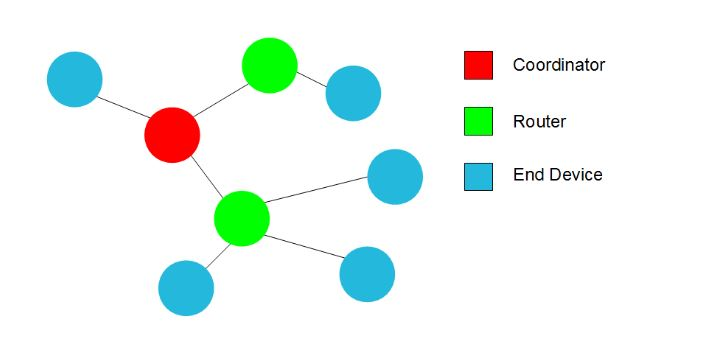
\includegraphics[width=0.5\linewidth]{mesh.jpg}
		\caption{Mesh Network Visualized}
		\label{fig:mesh}
	\end{figure}
	\subsection{Creating the Wireless Network between the Coordinator and Router modules}
	\par We wanted to create a wireless network between the coordinator and router modules this time. Firstly, we started off with soldering our XBee Explorer to connect our router modules on top of them. The reason we chose Xbee Explorer was because it will allow us to solder the input power voltage and the output pins that will be connected to the sensors. We used the application XCTU to help us set up each Xbee as a coordinator or router modules. We first set our coordinator in API mode that will allow us to communicate directly with the sensors via router modules. At the same time, we set the other three router modules to be in a AT or Transparent mode. This will allow sensors to send data directly to the coordinator. We also made sure all the XBee modules used the same Channel and Personal area network (PAN) ID. 
	\begin{figure}[h]
		\centering
		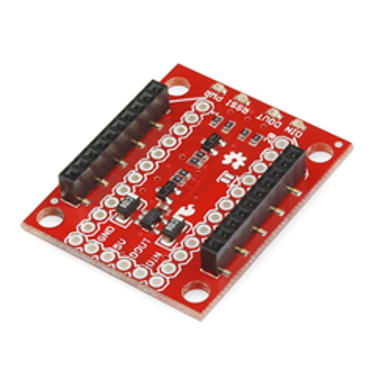
\includegraphics[width = 0.3\textwidth]{xbeeMiniExplorer.png}
		\caption{Small XBee interface to be used in each module}
	\end{figure}
	\subsection{Controlling the Router XBee with XCTU Remote AT Command}
	\par We decided to test our router XBee remotely by sending some AT Commands. We used the XCTU application to first create the Remote AT Command to turn on and off pin 18 of the router XBee. To see if we receive any output, we put an LED to see if the pin was turned on or not. In the figure below you can see the LED turning on and off via Pin 18 of the XBee device. The pictures help visualize what the pin is doing corresponding to the LED.
	\begin{figure}[h!]
		\centering
		\begin{subfigure}[t]{0.22\textwidth}
			\centering
			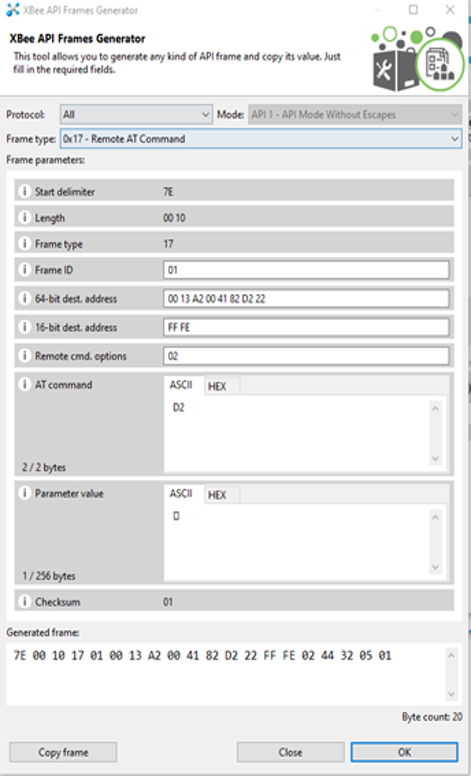
\includegraphics[width=\textwidth]{xbeeXctu1.png}
			\caption{Turn On Pin 18}
		\end{subfigure}
		\begin{subfigure}[t]{0.22\textwidth}
			\centering
			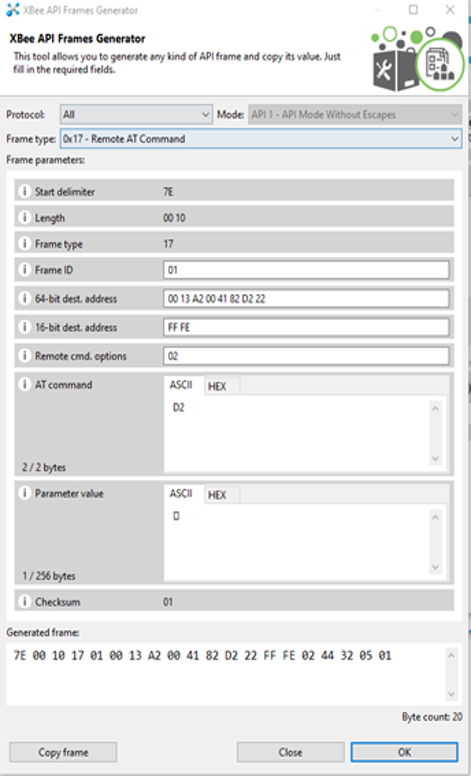
\includegraphics[width=\textwidth]{xbeeXctu1.png}
			\caption{Turn Off Pin 18}
		\end{subfigure}
		\caption{Simple LED activation over 802.15.4}
	\end{figure}
	\begin{figure}[h!]
		\centering
		\begin{subfigure}[t]{0.45\textwidth}
			\centering
			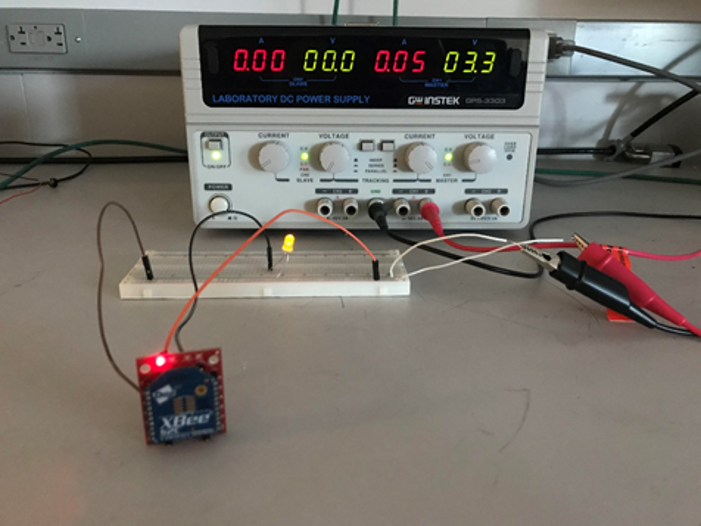
\includegraphics[height=1.5in]{ledRemoteTest.png}
			\caption{LED on via pin 18}
		\end{subfigure}
		\begin{subfigure}[t]{0.45\textwidth}
			\centering
			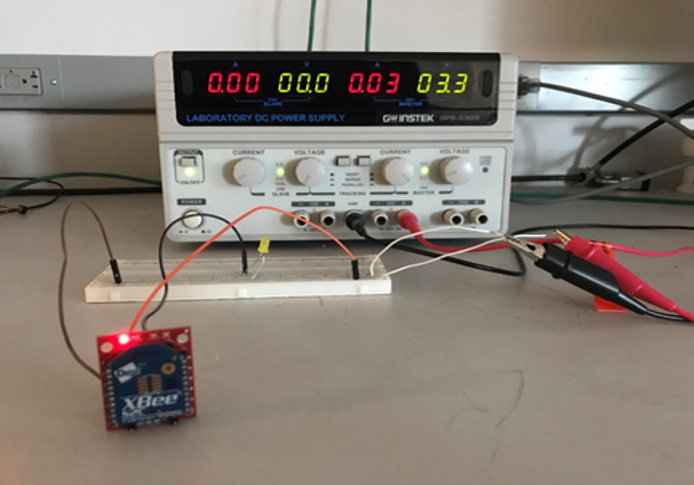
\includegraphics[height=1.5in]{ledRemoteTestOFF.png}
			\caption{LED off via pin 18}
		\end{subfigure}
		\caption{Simple LED activation over 802.15.4 (2)}
	\end{figure}
	\subsection{XBee Digital In/Out setup \textit{(DIO)}}
	\par The XBee devices have the capability to detect a change in a digital input signal. This edge detection allows the remote motion sensing module to transmit its data only if the signal changes. The coordinator will receive two packets, the first being a reading of logic high, the second being a reading of logic low once the sensor has stopped detecting any movement. In this way the unit does not need to send samples at a continuous rate, which saves power.
	\par To enable the change detection feature on DIO3, we need to set the hexadecimal value in the setting DIO change detect to 0x4. As seen on the right side of Figure \ref{fig:changeDet} this will enable the change detection on bit 2 only, which corresponds to DIO3. 
	\begin{figure}[h]
		\centering
		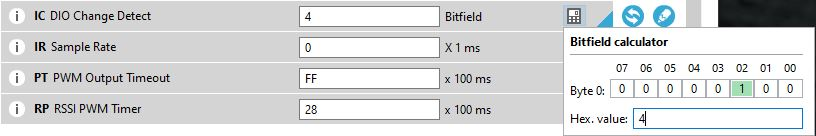
\includegraphics[width=0.8\linewidth]{changeDetect.JPG}
		\caption{Change detection parameters in XCTU}
		\label{fig:changeDet}
	\end{figure}
	\par When initially attempting to read data from the XBee's DIO pin, the value read would always read high. This reading was verified with a multimeter as well as on the scope. After some trouble shooting it was discovered that the issue lie in the I/O settings of the XBee, which has the ability to pull its digital inputs or outputs high or low based on a bit mask. 
	\begin{figure}[h]
		\centering
		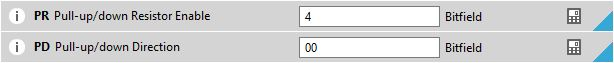
\includegraphics[width=0.8\linewidth]{bitMask.JPG}
		\caption{Bit masking settings for pull-up/pull-down resistors.}
		\label{fig:bitMask}
	\end{figure}
	\par In XCTU the mask had been set to pull all DIO pins high, which was not allowing a low input to be seen. Once re-masked, pulling the DIO pin used for the sensor reading down by default, the values were read correctly.
	
	\subsection{Digital I/O Interfacing with Python}
	The next step was to interact with the system through via python. After some initial testing of functions and learning the syntax a small GUI (Figure \ref{fig:motGui}) was created to display red when tripped and green when no movement was present. 
	\begin{figure}[h]
		\centering
		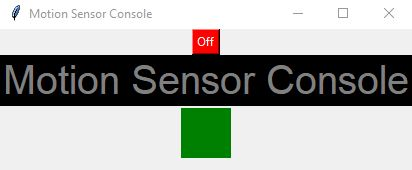
\includegraphics[width=0.5\linewidth]{motionGui.jpg}
		\caption{Motion Sensor Interface}
		\label{fig:motGui}
	\end{figure}
\newpage
	\begin{lstlisting}
		# setup gui elements ---------
		
		window = tk.Tk(screenName="Test Name", baseName=None, className='Tk', useTk=1)
		window.title("Motion Sensor Console")
		motion_canvas = tk.Canvas(window, bg="green", width=50, height=50)
		btn_ON_OFF = tk.Button(window,
							   activebackground="grey",
							   text="Off",
							   fg='white',
							   bg='red'
							  )
		# window title banner
		window_banner = tk.Label(window,
								 text="Motion Sensor Console",
								 fg='grey',
								 bg='black',
								 relief="solid",
								 font=("Arial", 30, "normal")
								)
	\end{lstlisting}
		Then, by establishing a serial connection with the coordinator, the whole network can be controlled and modified from a python program. Reading the digital input from the remote sensor, its is converted into a usable format, and if a rising edge was detected the program enter the triggered state and display a a red block. When a falling edge is received, the program will reset to a normal state. 
	\subsection{Primary GUI}
			\par This graphical user interface (GUI) was simply developed as a user friendly software. This allow users to operate and control electronic device through manipulation of buttons, gestures, and mouse. In our project, the users would have the capability of turning on/off the system, control the cameras, and turn on/off the alarm. The users have this feature for their ease and comfort. This can act accordingly to any difficult situations. The code below is a prototype of the GUI we were thinking of.  
			\begin{lstlisting}
			labell=Label(window,text="HOME AUTOMATION", fg='blue', bg='yellow', 
			relief="solid", font=("stencil",30,"bold")).place(x=139,y=22)
			
			#def main():
			#print('OLA')
			
			button1: Button=Button(window,text="TURN ON SYSTEM",fg='red', bg='purple',
			relief=RAISED,font=("arial",14,"bold"))#,command=main())
			button1.place(x=100,y=90)
			button1.config(height=3, width=22)
			
			button2=Button(window,text="TURN OFF SYSTEM",fg='red',bg='brown',
			relief=RAISED,font=("arial",14,"bold"))
			button2.place(x=300,y=90)
			button2.config(height=3, width=22)
			
			button3=Button(window,text="TURN ON ALARM",fg='red',bg='brown',
			relief=RAISED,font=("arial",14,"bold"))
			button3.place(x=100,y=165)
			button3.config(height=3, width=22)
			
			button4=Button(window,text="TURN OFF ALARM",fg='red',bg='brown',
			relief=RAISED,font=("arial",14,"bold"))
			button4.place(x=300,y=165)
			button4.config(height=3, width=22)
			
			button5=Button(window,text="TURN ON CAMERA",fg='red',bg='brown',
			relief=RAISED,font=("arial",14,"bold"))
			button5.place(x=100,y=238)
			button5.config(height=3, width=22)
			
			button6=Button(window,text="TURN OFF CAMERA",fg='red',bg='brown',
			relief=RAISED,font=("arial",14,"bold"))
			button6.place(x=300,y=238)
			button6.config(height=3, width=22)
			
			window.mainloop()
			\end{lstlisting}
			\begin{figure}[h]
				\centering
				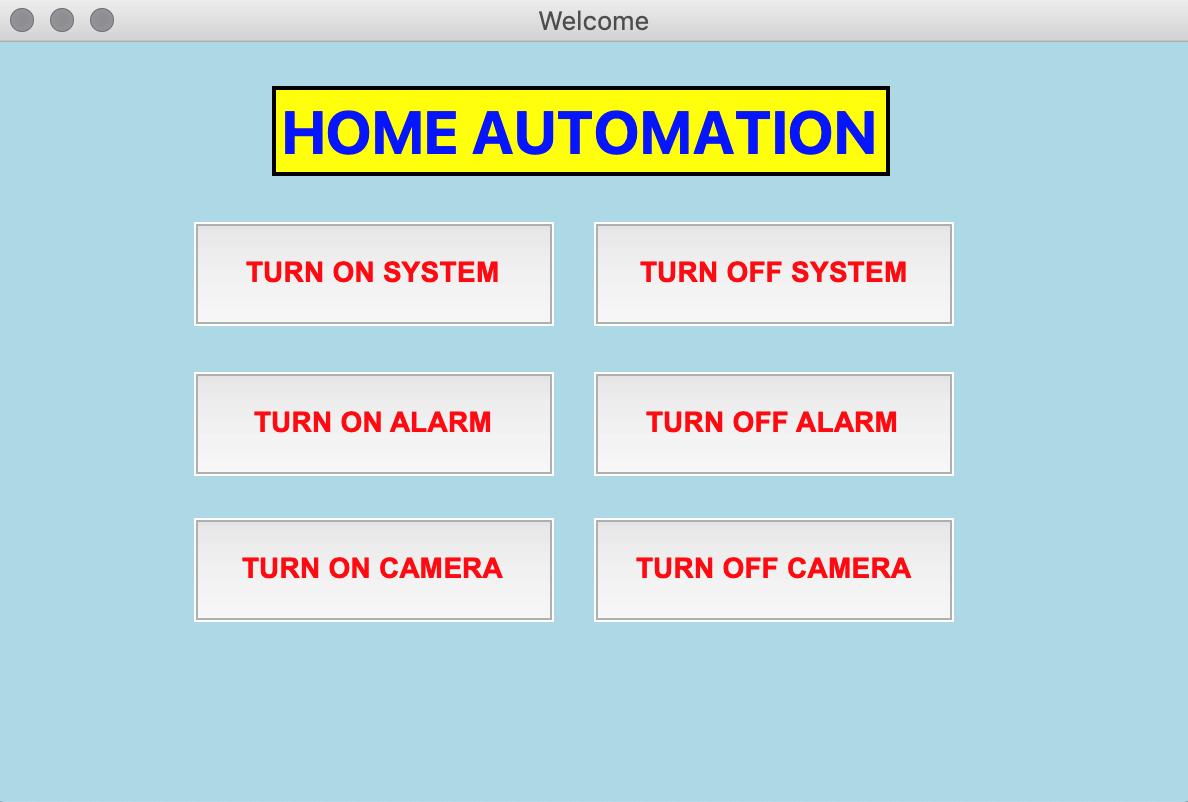
\includegraphics[width=0.75\linewidth]{gui.png}
				\caption{Main System GUI}
				\label{fig:maingui}
			\end{figure}
					
		\par When using a GUI in python the window runs in an infinite loop, constantly updating. This prevents the program from executing anything while the \textit{"mainloop()"} is running. To avoid this issue. The gui will setup the window environment and then enter a recursive function that reads and interpenetrates the digital data being received and updates the window elements accordingly. 
		\begin{lstlisting}
			window_banner.pack()
			motion_canvas.pack()
			print("re-paint")
			window.update()
			print("set window interrupt")
			window.after(0, get_motion_status()) # recursive function
		\end{lstlisting}
		\par If the remote module was sending samples at a constant rate this is much simpler, missed packets are less of a concern. The change detect digital IO configuration will only send a data packet when an event occurs. This means that the python program must spend most of its time waiting for data to arrive from the serial port. By setting a timeout in the serial setup, the program will wait for data for a set time before executing the rest of the loop. If the timeout was indefinite the window would not update properly. If the timeout is too short, the program will miss packets that arrive while the rest of the function is executing. With a timeout slightly less that the 2 second high-time of the sensor itself, the program spend the majority of its time listening for data and will miss very few data transmissions, while still updating the window elements at a reasonable rate.\\
		The below code block shows the recursive function written to check for motion sensor data and update the display:
		\begin{lstlisting}
			def get_motion_status():
				data_raw = ''
				initial_red_time = 0
				ser1 = serial.Serial('COM3', 9600, timeout=1.75)
				data_raw = ser1.read(14)
				
				if data_raw == '':
					ser1.close()
					window.after(0, get_motion_status())
					window.update()
				else:
					try:
						data_hex = binascii.hexlify(data_raw).decode('utf-8')
						D2 = data_hex[22:26]  # extract desired bits
						base_ten_val =int(D2, 16)
						# print("this sample:")
						print(base_ten_val)  # view data
					
					except ValueError:
						# print("caught valueError")
						ser1.close()
						# print("re-paint")
						window.update()
					
					else:
						print("Data received")
						if base_ten_val == 4:
						print("set indicator: red")
						motion_canvas.config(bg="red")
						print("re-paint")
						initial_red_time = time.now()
						window.update()
						elif base_ten_val == 0 or '':
						print("set indicator: green")
						motion_canvas.config(bg="green")
						print("re-paint")
						initial_red_time = 0
						window.update()
					finally:
						ser1.close()
						# print("re-paint")
						window.update()
						# print("set window interrupt")
						window.after(0, get_motion_status())
		\end{lstlisting}
		
		\begin{figure}[h]
			\centering
			\begin{subfigure}[t]{0.4\textwidth}
				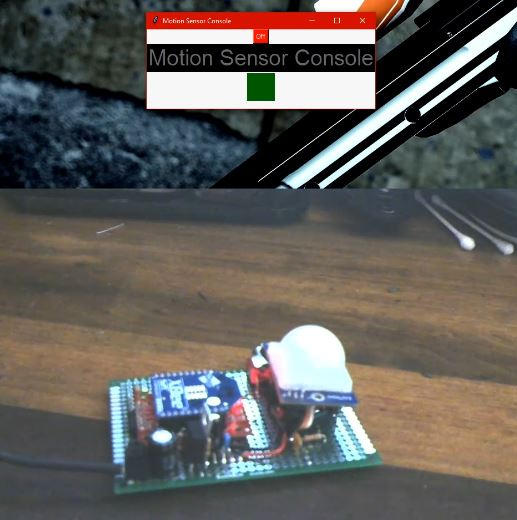
\includegraphics[width=\textwidth]{motionOff.JPG}
				\caption{Safe}
			\end{subfigure}
			\begin{subfigure}[t]{0.4\textwidth}
				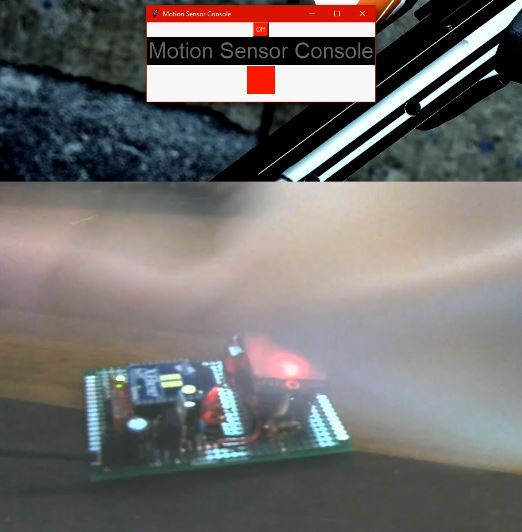
\includegraphics[width=\textwidth]{motionOn.JPG}
				\caption{Triggered}
			\end{subfigure}
			\caption{Motion Sensor GUI functionality}
			\label{fig:motionFunc}
		\end{figure}
		
		\par To account for any data that is missed a contingency was added to the program such that if the program is in the "tripped" state for too long it will automatically reset to "safe." If the sensor is being tripped it will be set to the "tripped" state again almost immediately. Remaining tripped for too long indicate that a rising edge was received but a falling edge was not. If no movement occurs after a missed falling edge the program would remain in the tripped state indefinitely.
		\begin{lstlisting}
			delta_t = time.now() - initial_red_time
			threshold_time = time.time(0, 0, 10)    # threshold for missed low == 10 sec
			
			if delta_t - threshold_time < 0:
				"""IF time after a high signal received exceeds 10 seconds, reset. If a falling edge missed program will remain high until the falling edge of subsequent trigger. If tripped value will return to tripped state on the next loop until 10 seconds have passed again. """
			
				print("set indicator: green")
				motion_canvas.config(bg="green")
				print("re-paint")
				initial_red_time = 0
				window.update()
		\end{lstlisting}
		
	
	\subsection{Controlling XBee module using Python}
	\par Since we now know that remote router XBee can be controlled by the coordinator XBee wireless, we decided to use python program for the same task. First, we connected our coordinator XBee module to the computer and set it to API mode. Then we powered up the router module and now we know that it has been connected in a wireless mesh network. We used the XCTU application to generate the same Remote AT Command frame to control the pin 18 of the router module. Then opened the python program to start writing our program in a new script file. API frame generated to Turn on \& Off pin 18: 
	\begin{figure}[h!]
		\centering
		\begin{subfigure}[t]{0.22\textwidth}
			\centering
			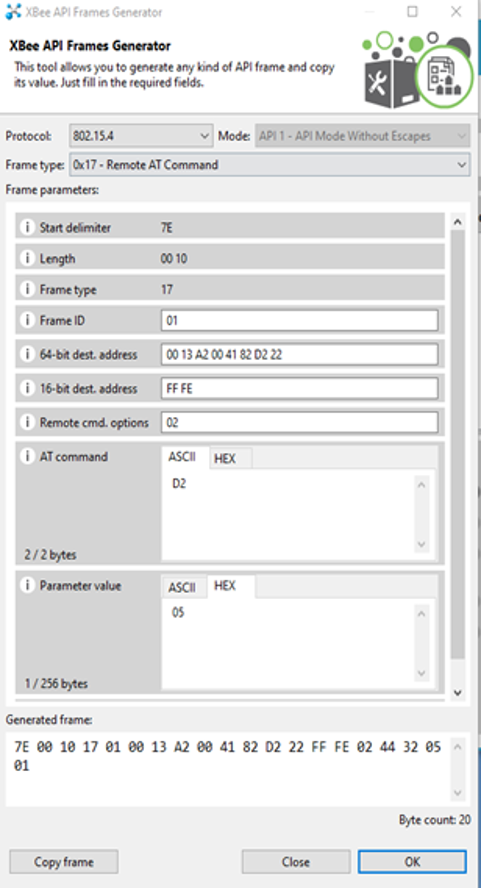
\includegraphics[width=\textwidth]{xctuFrames1.png}
			\caption{Turn On Pin 18}
		\end{subfigure}
		\begin{subfigure}[t]{0.22\textwidth}
			\centering
			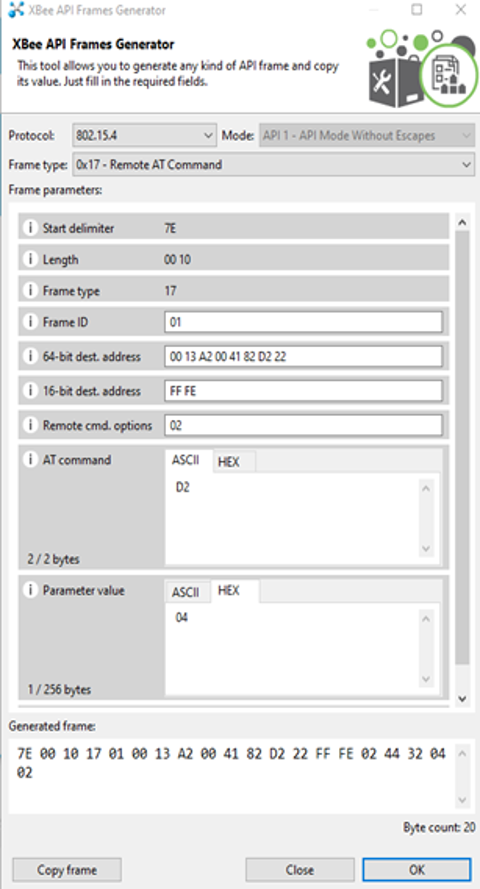
\includegraphics[width=\textwidth]{xctuFrames2.png}
			\caption{Turn Off Pin 18}
		\end{subfigure}
		\caption{API Frames created in XCTU}
	\end{figure} 
	\begin{lstlisting}
	#Configure AD2 and DIO2 to control pin-18
	
	import serial
	import binascii
	import time
	
	ser = serial.Serial(COM3)
	ser.baudrate = 9600
	
	#XCTU API Frame remote AT command used to control pin-18
	#Power ON
	turnOn = "7E 00 01 17 01 00 13 A2 00 41 82 D2 22 FF FE 02 44 32 05 01"
	#Power OFF
	turnOff = "7E 00 01 17 01 00 13 A2 00 41 82 D2 22 FF FE 02 44 32 04 02"
	
	#Use binascii to convert hex instruction to binary
	messageOn = "".join(turnOn.split()) 
	on = binascii.unhexlify(messageOn)
	
	messageOff = "".join(turnOff.split())
	off = binascii.unhexlify(messageOff)
	
	#Test write commands, flash led at 5 sec intervals
	count = 0
	while (count < 10)
		ser.write(on)
		time.sleep(5)
		ser.write(off)
		count = count + 1
	\end{lstlisting}
	
	\subsection{Gas Sensor Interfacing \& Data Processing}
		Since the MQ-6 LPG sensor is an analog device, all sampled data must be converted to digital data by an analog to digital converter before transmission. As a result of this, all data received by python will be binary voltage values which must be converted into a usable format. 
		\subsubsection{Threshold Detection}
			\par After the sensor started to give us the correct voltages, we decided to use python interface to plot us few graphs for us in real time. This way we have more visual knowledge and meaning about the data the sensor is sending to us. The code to plot graph is shown below.
			\begin{lstlisting}
			#initializing the function to open the XBee Coordinator		
			ser1=serial.Serial()		
			ser1.baudrate=9600  #speed		
			ser1.port='COM3'    #port address
						
			#figure for plotting the Time Vs Votlage			
			fig = plt.figure()			
			ax=fig.add_subplot(1,1,1)
						
			time=[]			
			volt=[]
						
			#open the serial port of the coordinator for incomming signal from the gas sensor			
			ser1.open()
					
			#Periodically from funcAnimation			
			def animate(i,time,volt):			
				data=ser1.read(14)			
				v=binascii.hexlify(data).decode('utf-8') #decode the data to Hexadecimal			
				D2=v[22:26]                              #select the Voltage range from the Hexadecimal
				Dec2=int(D2,16)                          #covert the Hexadecimal to Decimal value			
				Voltage=1.2*Dec2/1023                    #formula to finally to convert decimal to voltage reading
							
				time.append(dt.datetime.now().strftime('%H:%M:%S')) #Display current time 			
				volt.append(Voltage)
						
				time=time[-20:] #Trim and updated the 20 cureent incoming data 			
				volt=volt[-20:] #Trim and updated the 20 cureent incoming data 
				
				#Below is the style, axis label, and intervals for the graph
				ax.clear()
			    ax.plot(time,volt) 				
				plt.plot()				
				plt.xticks(rotation=45, ha='right')				
				plt.subplots_adjust(bottom=0.30)				
				plt.title('Voltage over Time')				
				plt.ylabel('Voltage(V)')				
				plt.xlabel('Time')				
				plt.ylim(0,1.3)				
				plt.grid(color='black',linestyle='dotted')
				plt.axhline(0.35)
				
				ani=animation.FuncAnimation(fig,animate,fargs=(time,volt), interval=1000)
				plt.show()
				ser1.close()
			\end{lstlisting}
		\subsubsection{Finding the Average, Mean, and Variance of sampled voltages}
			\par The voltages we were receiving from the sensor were finally what we expected. Our next goal was to find the threshold of the sensor so that we could make a visual cut off of the concentration of gas in terms of PPM and voltages in real time. We started off my reading the voltages from the sensor and computing the mean, average, and variance from the sensor directly.\\
			The following Program was written to attain these values: \\
			\begin{lstlisting}
				#Importing the modules				
				import serial				
				import binascii				
				import time				
				import numpy as np
								
				#initializing the function to open the XBee Coordinator				
				ser1=serial.Serial()				
				ser1.baudrate=9600   #speed				
				ser1.port='COM3'     #port address				
				ser1.open()          #open port
								
				#For Loop to keep reading data			
				for i in range(15):				
				data=ser1.read(14)				
				v=binascii.hexlify(data).decode('utf-8') #decode the data to Hexadecimal				
				print(v)
								
				D2=v[22:26]  #Select the Voltage range from the Hexadecimal				
				Dec2=int(D2,16) #covert the Hexadecimal to Decimal value 			
				print(D2)				
				
				Voltage=1.2*Dec2/1023  # formula to finally to convert decimal to voltage reading												
				print(volt)				
				
				average=np.average(volt)  #compute the average of the voltages				
				mean=np.mean(volt)        #compute the mean of the voltages
				vari=np.var(volt)         #compute the variance of the voltages

				print('The Average of the Sensor is:')
				print(average)
				print('The Mean of the Sensor is:')
				print(mean)
				print('The Variance of the Sensor is')
				print(vari)
				
				ser1.close()         #close port
				########################################
				Output:
					The Average of the Sensor is:
					0.255
					The Mean of the Sensor is:
					0.255
					The Variance of the Sensor is:
					0.0
			\end{lstlisting}
			\subsubsection{Calculating True Parts-Per-Million \textit{(PPM)}}
				\par Parts per million is very useful way of describing small amounts of concentration compared to the larger amount of concentration. In our project we will be using PPM to compare our concentration of any type of gas from our MQ-6 sensor. We are mainly targeting LPG.
				\par Using documentation provided in the manufacturer data sheet (MDS) for the MQ-6 (Appendix \ref{app:mq6}) the system can be calibrated to read a very accurate PPM of select ambient gasses.
				\begin{figure}[h]
					\centering
					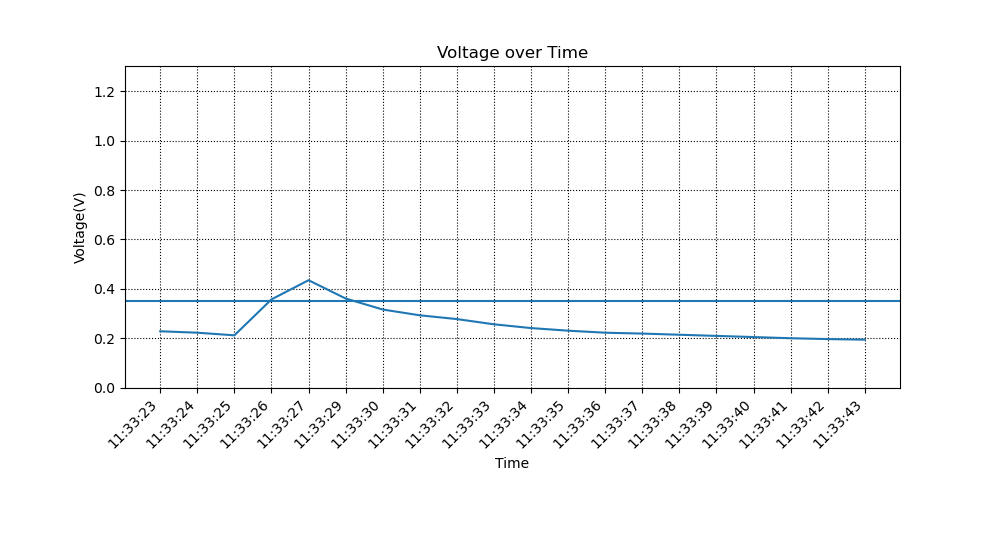
\includegraphics[width=\linewidth]{thdDetect.png}
					\caption{One of several sets of data, Live python plot}
					\label{fig:angGraph}
				\end{figure}
				\par The ordinate is resistance ratio of the sensor (Rs/Ro)  the abscissa is concentration of gases. Rs means resistance in target gas with different concentration, R0 means resistance of sensor in clean air. All tests are finished under standard test conditions. The x axis is in ppm while y axis is $\frac{R_s}{R_o}$. This ratio can be calculated using Equation \ref{eqn:ratio1}, where m is the slope and b is the y- intercept which can be solved using any two points from the graph in Figure \ref{fig:angGraph}, see Table \ref{tab:ppmEx}. \\
				\begin{equation}
				Log_10(\frac{R_s}{R_o}) = m\times Log_10(PPM) + b
				\label{eqn:ratio1}
				\end{equation}
				
				\begin{table}[h]
					\centering
					\begin{tabular}{ll}
						$\frac{R_s}{R_o}$ & PPM \\
						\hline
						1 & 1000 \\
						0.39 & 10,000 \\ 
						... & ... 
					\end{tabular}
				\caption{$\frac{R_s}{R_o}$ vs. PPM}
				\label{tab:ppmEx}
				\end{table}
				\par Using the Equation \ref{eqn:ratio1} with the values from Table \ref{tab:ppmEx} we can generate a system of two equations with which we can solve for $m$ and $b$. \\
				\begin{center}
					\small

						\[Log(1) = m \times Log(1000) + b  \]
						\[Log(0.39) = m \times Log(10,000) + b \]
						\[Solve:  \]
						\[m=-0.41,b=1.23\]
						Now we can solve for the PPM: \\
						\[Log(\frac{R_s}{R_o}) = m \times Log(PPM) + b \]
						\[\frac{R_s}{R_o} = 10^-0.41\times log(10) \times PPM + 1.23\]
						\[\frac{R_s}{R_o} = 10^1.23 \times 10^-0.41 \times log(10) \times PPM \]
						\[\frac{R_s}{R_o} = 16.982 \times PPM^-0.41 \]

				\end{center}
				\par Our main objective is to find a relation between the output sensor voltage $V_{out}$ and $\frac{R_s}{R_o}$. We start by assuming  that the circuit is made up of series resistance Rs and RL voltage divider of R1 and R2 as seen in Figure \ref{fig:resCirc} giving us equation \ref{eqn:resistance}. 
				\begin{center}
					\begin{figure}[h]
						\centering
						\includegraphics[width=0.5\linewidth]{resistCirc.JPG}
						\caption{Restive Circuit}
						\label{fig:resCirc}
					\end{figure}
					\small
					\begin{equation}
					\frac{V_1-V_s}{R_s}+\frac{V_1}{RL}+\frac{V_1-V_out}{R_1}=0
					\label{eqn:resistance}
					\end{equation}
					\[Known: R_1 = 16150\Omega, R_2 = 5100\Omega, RL = 20000\Omega, V_s = 5 v\]	
					\[\frac{V1-Vs}{Rs}+\frac{V1}{RL}+\frac{V1-Vout}{R1}=0\] 					
					\[\frac{V1}{RL}+\frac{V1-Vout}{R1}=-\frac{V1-Vs}{Rs}\] 					
					\[\frac{V1R1+V1RL-VoutRL}{R1*RL}=-\frac{V1-Vs}{Rs}\] 					
					\[Rs=-\frac{\left(V1-Vs\right)\left(R1*RL\right)}{V1*R1+V1*RL-Vout*RL}\] 					
					\[Rs=-\frac{\left(V1-Vs\right)\left(R1*RL\right)}{V1*R1+V1*RL-Vout*RL}\] 					
					\[Rs=-\frac{\left(V1*R1*RL-Vs*R1*RL\right)}{V1*R1+V1*RL-Vout*RL}\] 
					\begin{equation}
					Rs=\frac{Vs*R1*RL-V1*R1*RL}{V1*R1+V1*RL-Vout*RL}
					\label{eqn:resRatio}
					\end{equation}
				\end{center}
				From the graph, we can note that the resistance ratio in fresh air is a constant: \\
				\[R_s = R_o\]
				\par To find the Ro we will have to find the value of Rs in fresh air. So by taking the average of analog reading from the gas sensor and converting it into voltage reading, Average voltage reading from the sensor we found in clean air = 0.225 volts. \\
				Therefore: \\
				\[V1= \frac{R\mathrm{1+}R\mathrm{2}}{R\mathrm{2}}*\mathrm{Vout}\]
				\[V1= \frac{\mathrm{16150+5100}}{\mathrm{5100}}*0.225\]
				\[V1= 0.9375 volts\]
				Solving for Rs from equation \ref{eqn:resRatio} \\
				\[Rs=\frac{5*16150*20000-0.9375*16150*20000}{0.9375*16150+0.9375*20000-0.225*20000}\] 
				\begin{center}
				$Rs = 44645.9704\Omega = R_o $ (in clean air)
				\end{center}
				\par The value of Ro can be obtained only numerically. It is equal to the value of Rs in clean air condition. The value of Ro will remain constant and no need to be recomputed every time.
				Finally using equation \ref{eqn:ratio1} \\
				\[Log_10(\frac{Rs}{Ro}) = m\times log_10(PPM) + b\]
				\[m * Log(PPM) = Log_10(\frac{Rs}{Ro}) - b\] 
				\[\mathrm{PPM=\ }{\mathrm{10}}^{\ \ \frac{\mathrm{Log}\mathrm{10\ }\left(\frac{Rs}{Ro}\right)\mathrm{\ -\ b}}{m}}\] 		
				\[\mathrm{PPM=\ }{\mathrm{10}}^{\ \ \frac{\mathrm{Log}\mathrm{10\ }\left(\frac{Rs}{Ro}\right)\mathrm{\ -\ 1.23}}{-0.41}}\] 
				\[PPM=1000\]
				Where \\
				\[Ro=44645.9704\Omega  \]
				and \\
				
				\[\small Rs=\frac{Vs*R1*RL-V1*R1*RL}{V1*R1+V1*RL-Vout*RL}\] 
				
				\begin{center}
				 with changing $V_1$ \\
				\end{center}
				Therefore the PPM Equation will be,\\
				\[PPM = 10^\frac{Log_10(\frac{R_s}{R_o})-b}{m}\]
			
				
		
	